\section{Results} % min 7 pages
\label{sec:results}

I'll present here statistical and performance results from all of the implemented simulators. The specific parameters have been chosen differently for almost every graph in order to emphasize its characteristics. For more details check out all the different \texttt{main} scripts that can be found in GitHub's folder \texttt{Code/}. Important parameters that I kept constant are $M=8$ (the number of oscillators for the simulators. Note that for \textit{Clarke}'s simulator $N=M$, while for all the other \textit{SOS} simulators $N \approx 4M$) and the interpolation method (for \textit{Komninakis'} simulator) chosen to be \texttt{pchip}. With this, Matlab refers to a piecewise cubic polynomial interpolation with $C^1$ connections, instead of $C^2$ connection as for the more famous \texttt{spline}. A motivation for this choice will be given later on.

For all of the plots of the statistical results, a thick black line is firstly plotted with the ideal function, as described at the beginning of Section~\ref{subsec:math_models}.

%%%%%%%%%%%%%%%%%%%%%%%%%%%%%%%%%%%%%%%%%%%%%%%%%%%%%%%%%%%%%%%%%%%%%%%%%%%%%%%%%%%%%%%%%%%%%%%
%%%%%%%%% PDFs
%%%%%%%%%%%%%%%%%%%%%%%%%%%%%%%%%%%%%%%%%%%%%%%%%%%%%%%%%%%%%%%%%%%%%%%%%%%%%%%%%%%%%%%%%%%%%%%
\subsection{Probability Distribution Functions}

\begin{figure}
\hfill
\begin{minipage}{.49\linewidth}
	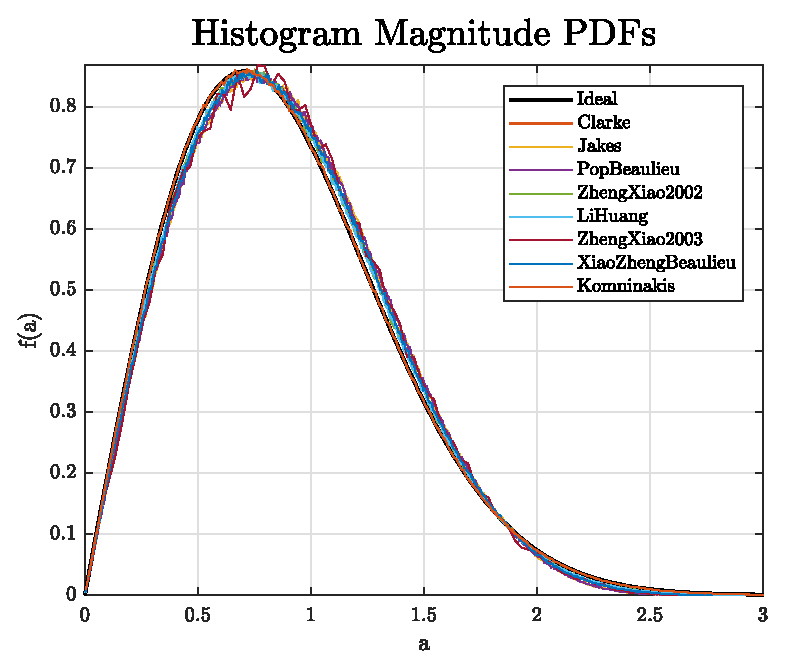
\includegraphics[width=\linewidth]{img/histMag.eps}
\end{minipage}
\hfill
\begin{minipage}{.49\linewidth}
	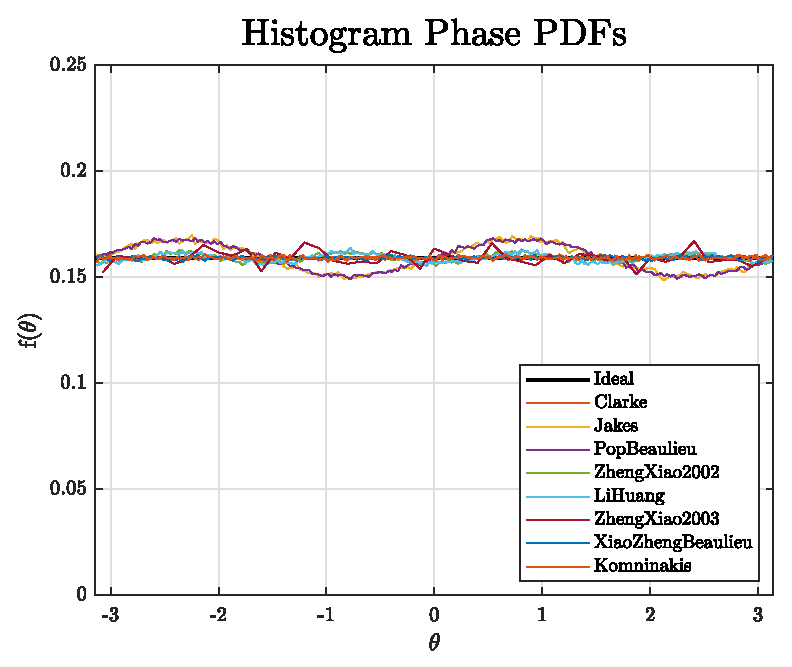
\includegraphics[width=\linewidth]{img/histPhase.eps}
\end{minipage}
\hfill

\caption{Histograms of Magnitudes and Phases of all the implemented simulators. Note the aforementioned problem with ZhengXiao2003}
\label{fig:histograms}
\end{figure}

The first results presented are simple Probability Distribution Functions, for both magnitude and phase of the channels. Assuming stationarity, many independent channels of every simulators were created and Matlab's \texttt{histogram} function was called on a specific samples across the channels. This was done to follow the probabilistic nature of the problem, avoiding the concept of ergodicity. One notable exception is \textit{Jakes'} simulator, which is fully deterministic, and thus its "PDF" was calculated on the single realization. Another exception to this rule is ZhengXiao2003: as it turns out, it is not really stationary. Calculating its PDF on the first sample, in fact, returned a very different result. In order to avoid this artifact, I created longer channels (about $T_{coh}$) and used the last sample instead. By doing this, though, I also had to provide less channels in order to not exceed memory limitations. The effect of this can be seen in Fig.~\ref{fig:histograms}, where ZhengXiao2003 has a rougher line.

Note, though, that all of the simulators approximate very accurately both PDFs (Eqs.~\ref{eqs:pdfs}), with the exception of \textit{Jakes'} and \textit{PopBeaulieu}'s simulators which clearly have an oscillatory behavior instead of a constant one for what concerns the phase PDF.

%%%%%%%%%%%%%%%%%%%%%%%%%%%%%%%%%%%%%%%%%%%%%%%%%%%%%%%%%%%%%%%%%%%%%%%%%%%%%%%%%%%%%%%%%%%%%%%
%%%%%%%%%%%% Correlations
%%%%%%%%%%%%%%%%%%%%%%%%%%%%%%%%%%%%%%%%%%%%%%%%%%%%%%%%%%%%%%%%%%%%%%%%%%%%%%%%%%%%%%%%%%%%%%%
\subsection{Correlations}

\begin{figure}
	\hfill
	\begin{minipage}{.49\linewidth}
		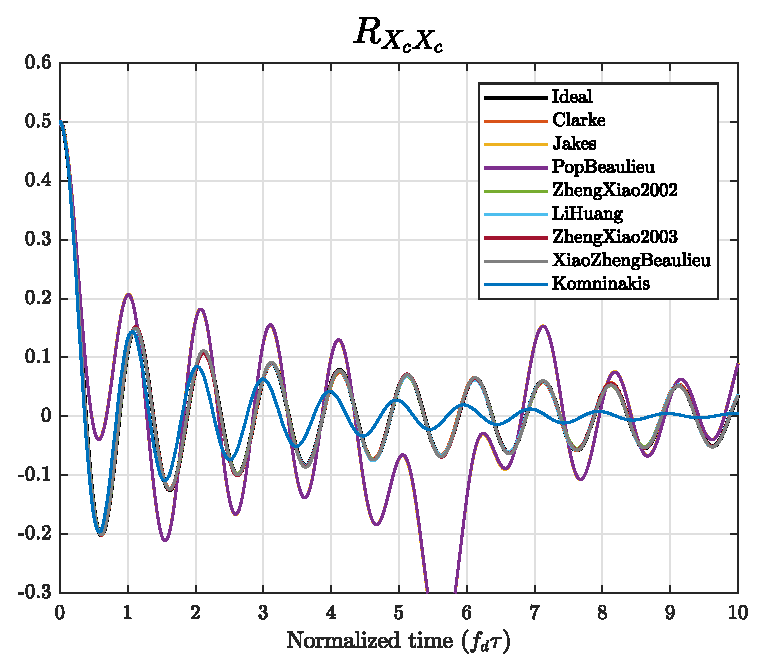
\includegraphics[width=\linewidth]{img/XcXc.eps}
	\end{minipage}
	\hfill
	\begin{minipage}{.49\linewidth}
		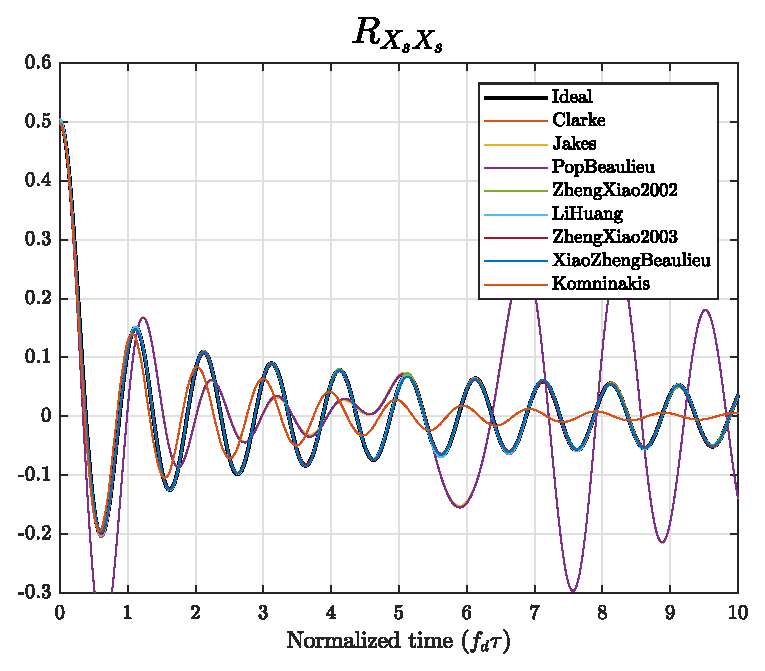
\includegraphics[width=\linewidth]{img/XsXs.eps}
	\end{minipage}
	\hfill
	
	\vspace{2mm}
	
	\hfill
	\begin{minipage}{.49\linewidth}
		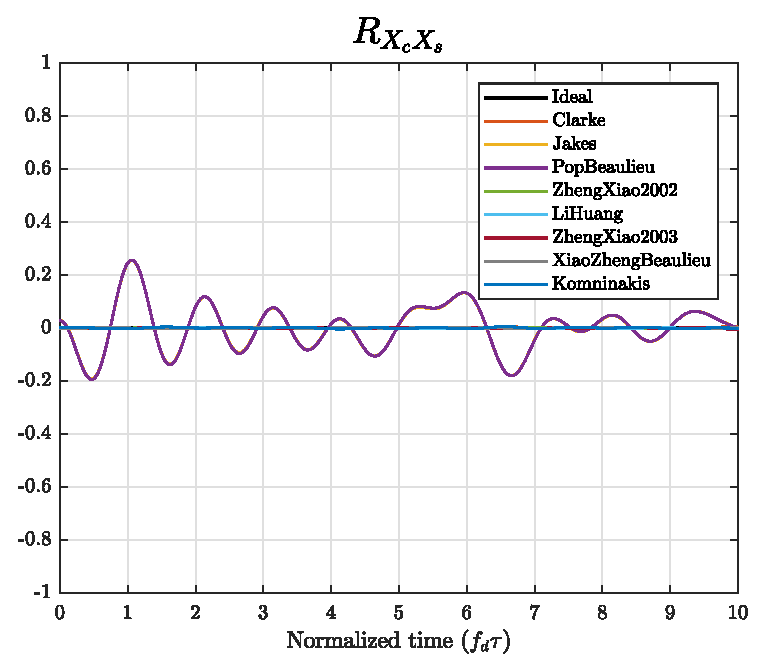
\includegraphics[width=\linewidth]{img/XcXs.eps}
	\end{minipage}
	\hfill
	\begin{minipage}{.49\linewidth}
		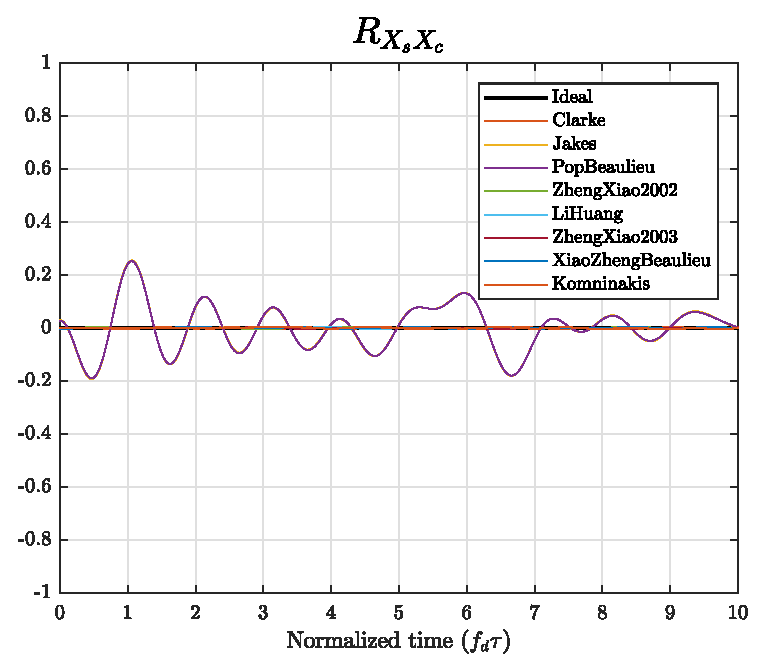
\includegraphics[width=\linewidth]{img/XsXc.eps}
	\end{minipage}
	\hfill
	
	\vspace{2mm}
	
	\hfill
	\begin{minipage}{.49\linewidth}
		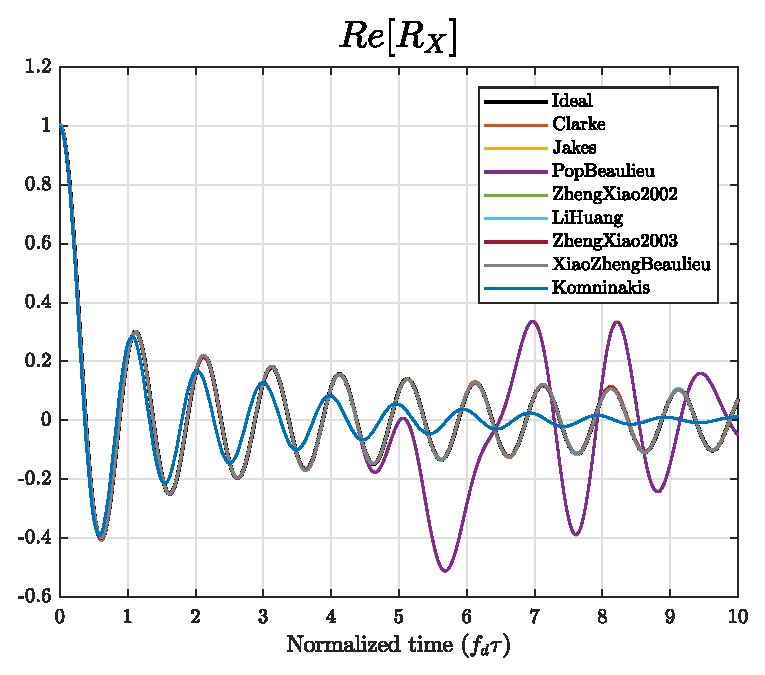
\includegraphics[width=\linewidth]{img/ReX.eps}
	\end{minipage}
	\hfill
	\begin{minipage}{.49\linewidth}
		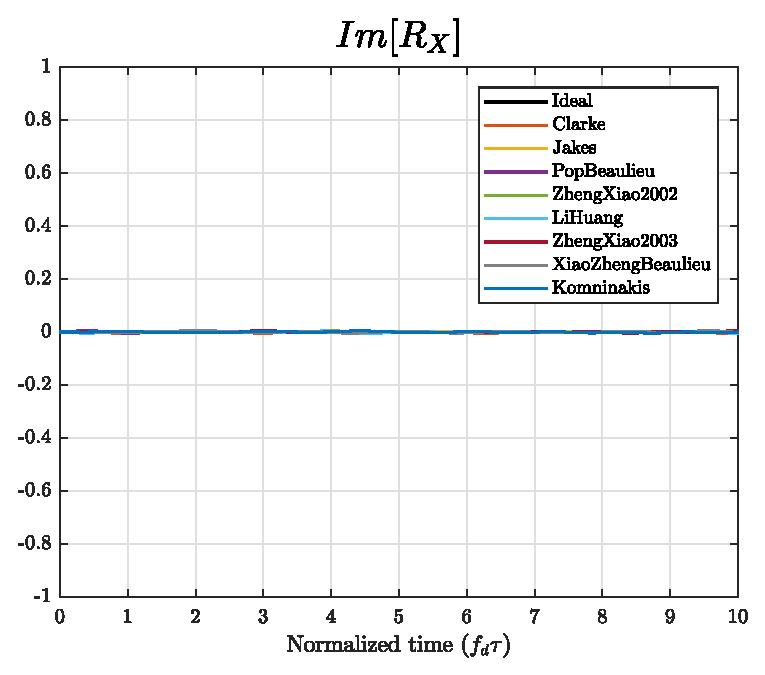
\includegraphics[width=\linewidth]{img/ImX.eps}
	\end{minipage}
	\hfill
	
	\caption{Cross correlations between real and imaginary components}
	\label{fig:xcorrs}
\end{figure}

Moving on to the correlations (Eqs.~\ref{eqs:correlations}, Figs.~\ref{fig:xcorrs}), it is clear that once again \textit{Jakes'} and \textit{PopBeaulieu}'s simulators cannot really match up with more modern solutions, resulting very early very imprecise especially when dealing with single real or imaginary components. For what concerns the correlation of the signal $X(t)$ as a whole, instead, they both tend to behave better, but still in the real part of $R_X$ they are both the first ones to significantly diverge from the ideal function.

\textit{Komninakis'} simulator is the other one that significantly diverges from the ideal case when non-zero functions are involved. Since its core idea is to design a filter that tries to mimic a given PSD (which I recall from \textit{Wiener–Khinchin theorem} is the \textit{Fourier Transform} of the autocorrelation function of the stochastic process), the reason why this happen should be a poor approximation of such filter. I also recall that I simply took the filter's coefficients from \cite{digital} without further investigations. It's clear from Fig.~\ref{fig:xcorrs}, though, that both the shape (quick ripple attenuation) and the Doppler frequency $f_d$ ("higher frequency" ripples) of the approximation are not really good.

All of the other simulators, instead, are almost indistinguishable from each other and from the ideal case, at least up to a normalized time $f_d\tau = 10$. I want to recall that this is obtained with only $8$ oscillators for all of these simulators! Note that also the original \textit{Clarke}'s simulator is indistinguishable from the ideal case with these few oscillators, and keep in mind that it's only a fourth of the equivalent number of oscillators simulated by the other designs. This is to empirically confirm the statement from \cite{B1} where \textit{Clarke}'s simulator is said to converge very quickly to the ideal case. This fact almost seems to suggest that \textit{Jakes'} simulator might not have been even needed in the first place!

\begin{wrapfigure}{R}{.45\linewidth}
	\centering
	\begin{minipage}{\linewidth}
		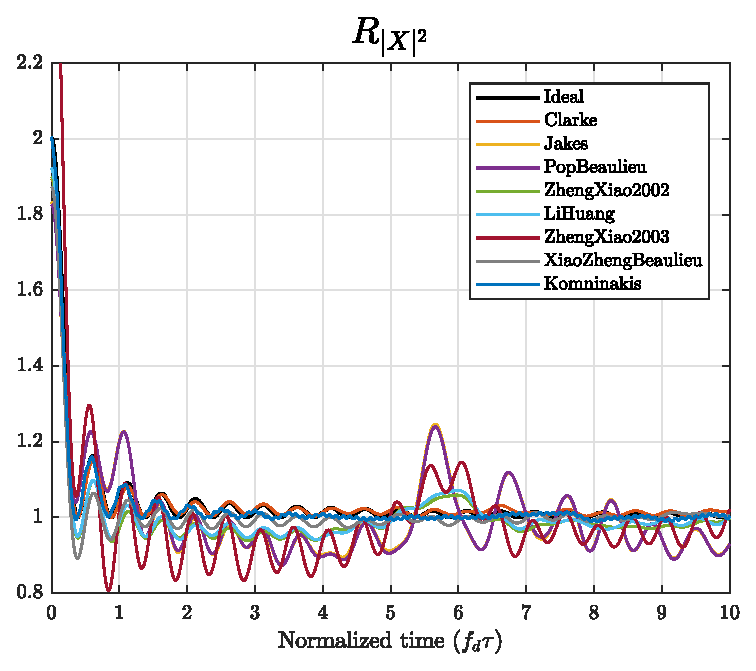
\includegraphics[width=\linewidth]{img/X2.eps}
	\end{minipage}
	
	\caption{Correlations of the channels}
	\label{fig:R_X2}
\end{wrapfigure}

One last correlation to consider is $R_{|X|^2}$, shown in Fig.~\ref{fig:R_X2}. Of all of the statistics shown up to now, this is definitely the most delicate one since it refers to powers (which is usually what we are really interested into) and in includes terms up to the fourth moment. Predictably it's the statistic that yields the worst results.

Once again, both \textit{Jakes'} and \textit{PopBeaulieu}'s simulators have among the worst statistics. In this case, \textit{ZhengXiao2003} yields quite bad statistics too. \textit{ZhengXiao2002}, \textit{LiHuang} and \textit{XiaoZhengBeaulieu}, instead are definitely an improvement. \textit{Komninakis} here is not bad, but has a strange ondulatory motion and, again, its oscillation seem to be too fast with respect to the ideal case. The clear winner, this time, is \textit{Clarke}'s simulator: even though it falls a bit short around the zero lag (about $1.9$ instead of $2$), the rest of the correlation is by far the closest of them all, and that's just with $8$ sinusoids!

%%%%%%%%%%%%%%%%%%%%%%%%%%%%%%%%%%%%%%%%%%%%%%%%%%%%%%%%%%%%%%%%%%%%%%%%%%%%%%%%%%%%%%%%%%%%%%%
%%%%%%%%%%%% LCR/AFD
%%%%%%%%%%%%%%%%%%%%%%%%%%%%%%%%%%%%%%%%%%%%%%%%%%%%%%%%%%%%%%%%%%%%%%%%%%%%%%%%%%%%%%%%%%%%%%%
\subsection{Fading Statistics}

\begin{figure}
	\hfill
	\begin{minipage}{.49\linewidth}
		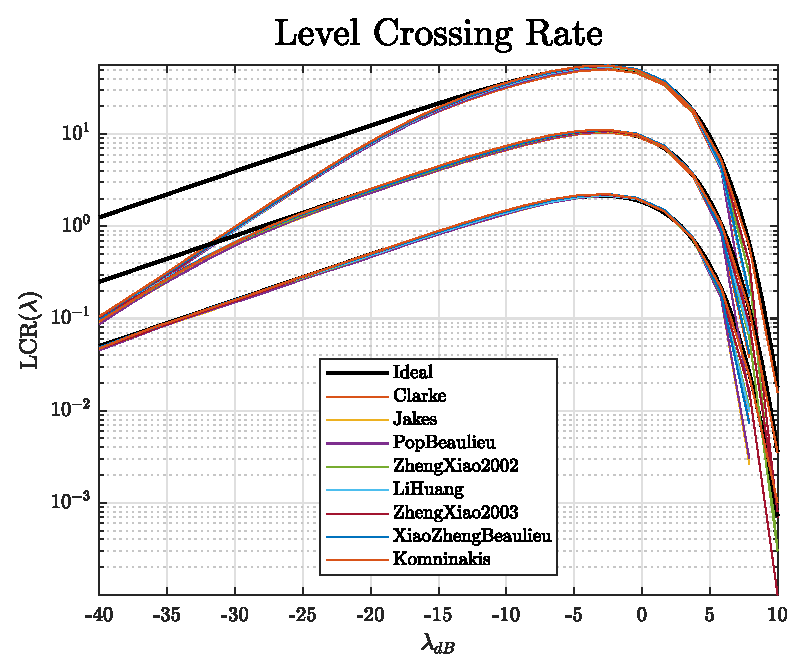
\includegraphics[width=\linewidth]{img/multiLCR.eps}
	\end{minipage}
	\hfill
	\begin{minipage}{.49\linewidth}
		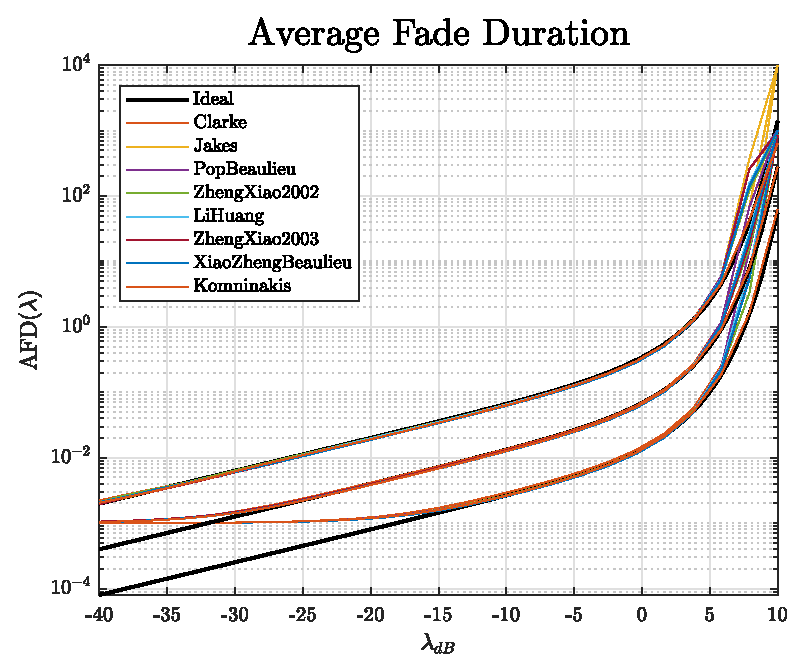
\includegraphics[width=\linewidth]{img/multiAFD.eps}
	\end{minipage}
	\hfill
	
	\caption{Plots for threshold-based statistics. Note that $\lambda_{dB} \triangleq 20\, \log_{10} \lambda$ since it's envelope related, not power related}
	\label{fig:LCR_AFD}
\end{figure}

The last statistics that I'm going to present here were not present in all of the reference papers, but i think they are really important if not crucial (for example in channel coding design). A short explanation and ideal formulas were given in Sec.~\ref{subsec:math_models}, Eqs.~\ref{eq:LCR},\ref{eq:AFD}.

Starting from \textit{LCR}, it is possible to see from Fig.~\ref{fig:LCR_AFD} how different values for $f_dT$ ($0.05$, $0.01$ and $0.002$) yield very different results. In particular for low thresholds, the higher $f_dT$ the earlier the deviation from the ideal formula begins. This can be seen in exactly the same way for all of the proposed simulators, hence it's probably caused by something more fundamental. Reference \cite{A3} attributes this phenomenon to the fact that for fast fading (or low sampling rate, i.e. a high value of $f_dT$), some very narrow troughs cannot be correctly sampled, thus giving an underestimate of the level crossing rate. As the fading slows down (or sampling rate increases, i.e. $f_dT$ decreases) more and more fine troughs can be correctly sampled. This, of course, only postpones the problem, but if the critical theshold is low enough for your specific purpose, the model works just fine.
For high thresholds, instead, there are some major differences among the simulators: here \textit{Komninakis} is definitely the best one being almost identical to the ideal curve up to $10$ dB. \textit{ZhengXiao2003} and \textit{ZhengXiao2002} are respectively the second and third best ones, but usually reaching the $10$ dB threshold about an order of magnitude lower. All the other simulators do not even register any crossing above $8$ dB. From $5$ dB and below, instead, they all perform perfectly. Note taht we are usually interested in low thresholds, since they are the ones responsible for errors, so the low precision towards higher levels may be considered on secondary importance.

Similar considerations can be done for the \textit{AFD}: an increasing $f_dT$ yields worst performance towards lower thresholds due to resoluation problems: in this case, a constant sampling period $T=1 ms$ was chosen, varying the Doppler spread as for the \textit{LCR} test. Note that the fade duration obviously cannot go below $1ms$, and higher/lower values of $f_dT$ make this problem arise sooner/later. Once again, \textit{Komninakis} tend to perform almost perfectly while all the others overshoot even considerably the ideal statistics. But still, we are usually interested for how long the channel will return erroneous bits, meaning for how long it will stay below a (low) threshold. So, as for the \textit{LCR}, also for the \textit{AFD} high levels may be considered not important and, again, it should be checked whether the product $f_dT$ is suitable for the particular problem.

%%%%%%%%%%%%%%%%%%%%%%%%%%%%%%%%%%%%%%%%%%%%%%%%%%%%%%%%%%%%%%%%%%%%%%%%%%%%%%%%%%%%%%%%%%%%%%%
%%%%%%%%%%%% Simulation Time
%%%%%%%%%%%%%%%%%%%%%%%%%%%%%%%%%%%%%%%%%%%%%%%%%%%%%%%%%%%%%%%%%%%%%%%%%%%%%%%%%%%%%%%%%%%%%%%
\subsection{Performance Evaluation}

\begin{figure}
	\hfill
	\begin{subfigure}[t]{.49\linewidth}
		\centering
		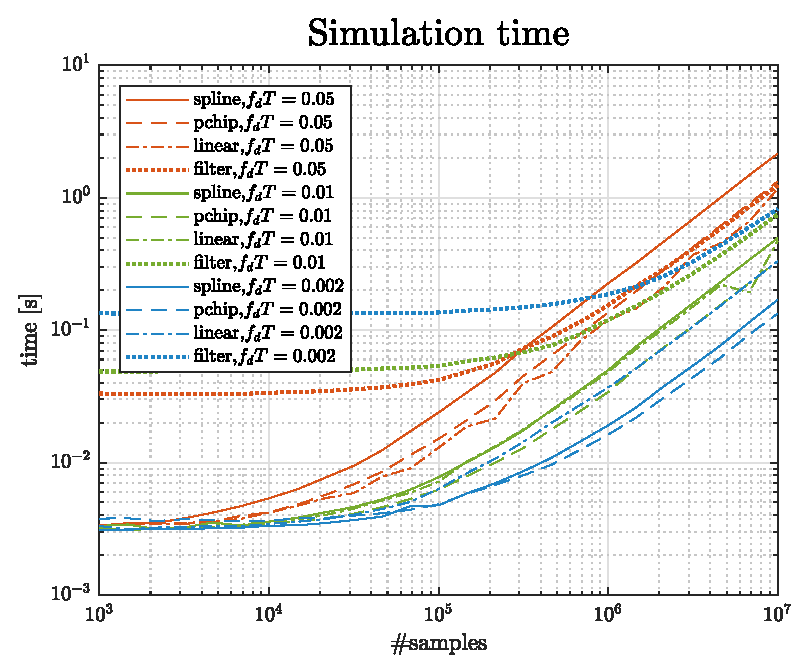
\includegraphics[width=\linewidth]{img/simTime_Komninakis.eps}
		\subcaption{Kominakis Simulation Time}
		\label{fig:KomninakisSimTime}
	\end{subfigure}
	\hfill
	\begin{subfigure}[t]{.49\linewidth}
		\centering
		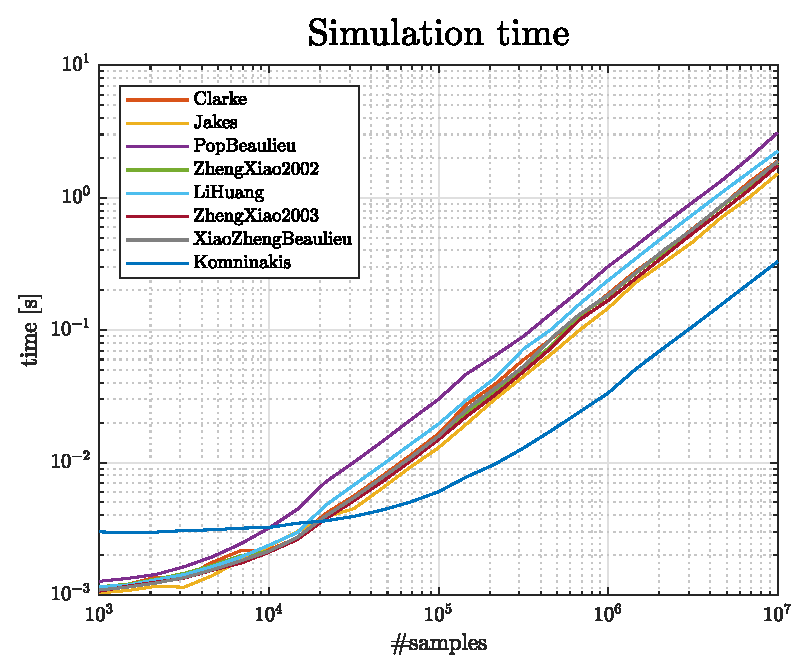
\includegraphics[width=\linewidth]{img/simTime.eps}
		\subcaption{Overall Simulation Time}
		\label{fig:overallSimTime}
	\end{subfigure}
	\hfill
	
	\caption{Simulation time for current implementations}
	\label{fig:simTime}
\end{figure}

\begin{wrapfigure}{R}{.45\linewidth}
	\centering
	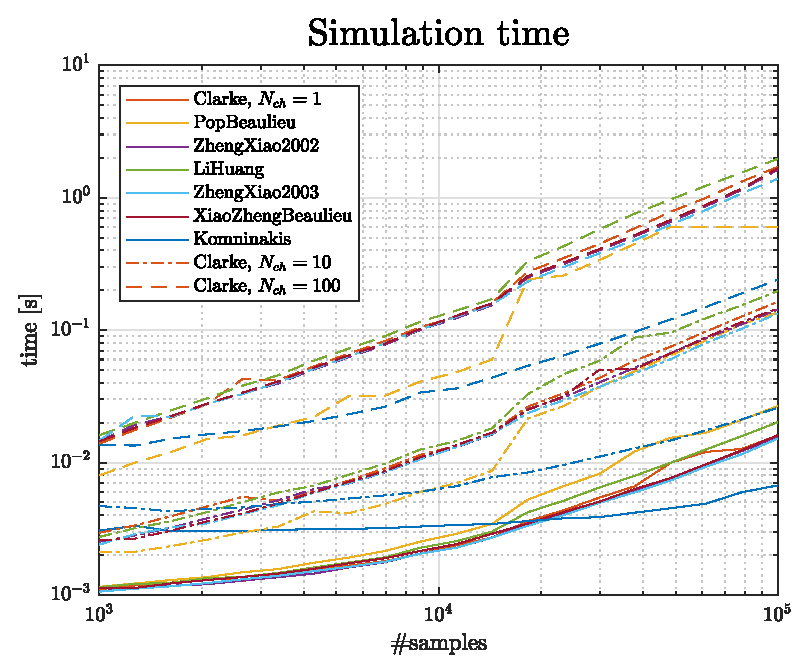
\includegraphics[width=\linewidth]{img/multiSimTime.eps}
	
	\caption{Simulation time with different number of channels}
	\label{fig:multiSimTime}
\end{wrapfigure}

One final test that i decided to do is a performance evaluation. This is quite delicate, though: a fine optimization should be carefully done for each one of the 8 simulators implemented in order to obtain meaningful results. Also, the results are machine and probably even CPU architecture dependent. In order to squeeze every last bit of performance, Matlab's proprietary profiler has been exploited over and over at the best of my capabilities for every simulator. For what concerns the architecture, Matlab R2017a has been used, running over a 64-bit Windows 10 machine equipped with an Intel Core i5-2500K (overclocked @4.11 GHz) and 8 GB of RAM. Each test has been carefully designed in order to maximize the memory usage without exceeding it (which would have artificially hurt performance). Finally, timings were taken through Matlab using the \texttt{tic-toc} instructions around a call to the function \texttt{createChannel}. Multiple simulations are then performed (at least 10) up until the $95\%$ \textit{Confidence Interval} falls below a $10\%$ error from the mean.

For the first test, I had to decide which type of interpolation for \textit{Komninakis}' simulator and $f_dT$ product to use for all of the previous tests. In Fig.~\ref{fig:KomninakisSimTime} how different $f_dT$ affect performance over a broad number of simulated samples. I want to recall that \textit{Komninakis'} filter is set to work at a fixed $f_dT=0.1$, hence for lower values of $f_dT$ a lower number of complex gaussian random variables will have to be created, a higher interpolation factor will be need and, thus, a narrower lowpass interpolation filter will have to be designed. This is perfectly reflected in the figure: for the filter interpolation, a much higher initial cost is needed in order to design the lowpass filter, and this cost raises the narrower the filter. For the polynomial interpolation, instead, no such cost is required thus yielding better performance when less random variables are needed (polynomial interpolation is low cost). Furthermore, the \textit{spline} interpolation, as expected, is the most expansive one, while \textit{pchip} is a bit more efficient. I expected \textit{linear} interpolation to be by far the most efficient one but apparently it is not so. In any case, statistics for this simple interpolation were quite bad, whereas \textit{spline} and \textit{pchip} were comparable. For the high initial cost, then, I didn't even considered the \textit{filter} method but it may be a possibility for a very high number of samples. For these reasons in the end I decided to use \textit{pchip} as the main interpolation method.

Looking, now, at Fig.~\ref{fig:overallSimTime}, the results for a single channel simulation, we clearly see two things at a glance: the \textit{Komninakis} simulator starts higher than the others but quickly surpasses them all, while they stay quite close to each other. The former is partially expected since it requires a much higher number of complex gaussian random variables while apparently \textit{pchip} interpolation is much faster than computing trigonometric functions, justifying the title of \cite{A3}. The latter is also quite expected, but maybe not this much close together. A few things to notice: \textit{Jakes'} simulator, fortunately, is the fastest one but \textit{PopBeaulieu} is by far the slowest one. Note also that \textit{Clarke}'s simulator doesn't perform so bad compared to the others.

One last curiosity that I had was about how simulators would beahve with a higher number of independent channels. Due to the deterministic nature of \textit{Jakes'} simulator, I did not include it in this comparison since it would have simple made a repetition of the first channel. I was able, though, to keep tha same colors for all the other simulators in oreder to have a better and unified visual presentation (Fig.~\ref{fig:multiSimTime}). The strangest result is certainly given by \textit{PopBeaulieu}: with only one channel it performs the worst while for 10 and 100 is actually the best one among the \textit{SOS} type of simulators, even with exceptional results up to $15 \cdot 10^3$ samples, then suddenly it aligns with the rest of the group. Here it can be fully appreciated the computational efficiency of \textit{Komninakis}' simulator: it can improve up to a full order of magnitude the simulation time!